\documentclass[10pt]{article}
\usepackage[utf8]{inputenc}
%\usepackage[T1]{fontenc}
\usepackage{tgbonum}
\usepackage[english]{babel}
\usepackage{graphicx}
\usepackage{amsmath}
\usepackage{amssymb}
\usepackage{hyperref}
\usepackage{epsf}
\usepackage{float}
\usepackage{mathpazo}
\usepackage{pifont}
\usepackage
[
a4paper,% other options: a3paper, a5paper, etc
left=2.2cm,
right=2.2cm,
top=2cm,
bottom=2cm,
]{geometry}
%\geometry{hmargin=3.5cm, vmargin=2.5cm}
\usepackage{fancyhdr}
\pagestyle{fancy}
\fancyhf{}
\rfoot{\thepage}
\renewcommand{\headrulewidth}{0pt}
\usepackage{color}
\usepackage{graphicx}
\usepackage{wrapfig}
\usepackage{graphicx}
\usepackage{multicol}
\usepackage{enumitem}
\usepackage{xcolor}
\usepackage{framed}
\usepackage{bm}
\definecolor{shadecolor}{RGB}{139, 231, 3}
\usepackage{epigraph}

\usepackage{tcolorbox}
\definecolor{mycolor}{rgb}{0.122, 0.435, 0.698}

\newtcbox{\mb}{nobeforeafter,colframe=mycolor,colback=mycolor!10!white,boxrule=0.5pt,arc=4pt,
  boxsep=0pt,left=6pt,right=6pt,top=3pt,bottom=3pt,tcbox raise base}

\usepackage{eso-pic}
\newcommand\BackgroundPic{%
\put(-0,-150){%
\parbox[b][\paperheight]{\paperwidth}{%
\vfill
\centering
\includegraphics[width=\paperwidth,%
keepaspectratio]{plots/foret-de-soignes.jpg}%
\vfill
}}}

\usepackage[T1]{fontenc}

\usepackage{anyfontsize}
\usepackage{t1enc}
\newcommand{\heart}{\ensuremath\varheartsuit}
\usepackage{tikz}
\usetikzlibrary{positioning}
\usepackage{charter}

\begin{document}

% TITLE PAGE ====================================================

\begin{titlepage}
\AddToShipoutPicture*{\BackgroundPic}
\ \\[4cm]
{\sffamily \color{white}
\begin{center}
\fontsize{34}{10}\selectfont \fontfamily{ppl}\selectfont Computational examples 

\fontsize{20}{10}\selectfont \fontfamily{ppl}\selectfont in 

\,\,\,

\fontsize{40}{10}\selectfont \fontfamily{ppl}\selectfont  transport phenomena

\,\,\,

\fontsize{25}{10} \selectfont \fontfamily{augie}\selectfont with Python

\end{center}
}
\vfill
{\fontsize{20}{20}\color{white}\sffamily Science Docs \hfill\color{white} Kamila Zdybał}

{\fontsize{10}{10}\color{white}\sffamily PDFs for explorers and experimenters}
\end{titlepage}


% EX LIBRIS PAGE ================================================

\thispagestyle{empty}
\begin{center}

This document was prepared as part of two courses from Delft University of Technology: \textit{The Basics of Transport Phenomena}, available on edX.org as DelftX: TP101x and \textit{Advanced Transport Phenomena}, available on edX.org as DelftX: TP201x.

This material was created by or adapted from material posted on the DelftX website, delftx.tudelft.nl, and created by TU Delft faculty members Robert Mudde, Professor of Multiphase Flow at the Dept. of Chemical Engineering and Peter Hamersma, Associate Professor at the Dept. of Chemical Engineering, 2015. DelftX is not responsible for any changes made to the original materials posted on its website and any such changes are the sole responsibility of Kamila Zdybał.

The course materials by Delft University of Technology are subjected to copyright and are licensed under a Creative Commons Attribution-NonCommercial-ShareAlike 4.0 International License.

https://creativecommons.org/licenses/by-nc-sa/4.0/

\vspace*{6cm}


\setlength{\parskip}{0.0em}
\setlength{\parindent}{0cm}

Copyright \textcopyright \, K. Zdybał, 2018, 2019

For more projects similar to this one

visit me on GitHub: \verb|@camillejr|

\verb|camillejr.github.io/science-docs/|

To contact me personally drop me a line at:

\verb|kamilazdybal@gmail.com|

\vspace*{1cm}

Cover picture: \textit{Forêt de Soignes, Belgium}

Photo taken on: 16 Jan 2017

Copyright \textcopyright \, K. Zdybał, 2017

\vspace*{6cm}

\verb|Computational examples in transport phenomena with Python|

Typeset with \LaTeX

\vspace*{2cm}

\noindent This work is licensed under the Creative Commons

Attribution-NonCommercial-ShareAlike 4.0 International 

(CC BY-NC-SA
4.0) license.

\end{center}
\setlength{\parskip}{0.6em}
\setlength{\parindent}{0.5cm}

\newpage

\tableofcontents

\newpage

\setlength{\parskip}{0.6em}
\setlength{\parindent}{0cm}


\,\,\,

\normalsize

\section{General remarks on transport of physical properties}

The general equation for the transport of a property $\psi$ within a control volume is:

\begin{equation}
\frac{d \psi}{dt} = \Psi_{in} - \Psi_{out} + \Psi_{production} - \Psi_{consumption}
\end{equation}

where $\frac{d \psi}{dt} = \dot{\psi}$ is the flux of the property $\psi$.

\newpage

\section{Steady-state conduction in a lengthwise-insulated rod with internal heat production}

We derive a one-dimensional temperature distribution function $T(x)$ for a steady-state heat conduction in a straight rod of length $L$. We assume that the internal heat production $Q_p$ in units of $W/m^3$ is present at every point inside the rod volume. This may for instance simulate heating up of a wire due to electrical current. The rod is perfectly insulated along its length and it loses heat only through its endpoints which in a steady-state case are kept at a fixed temperature $T_0$.

\begin{figure}[H]
\centering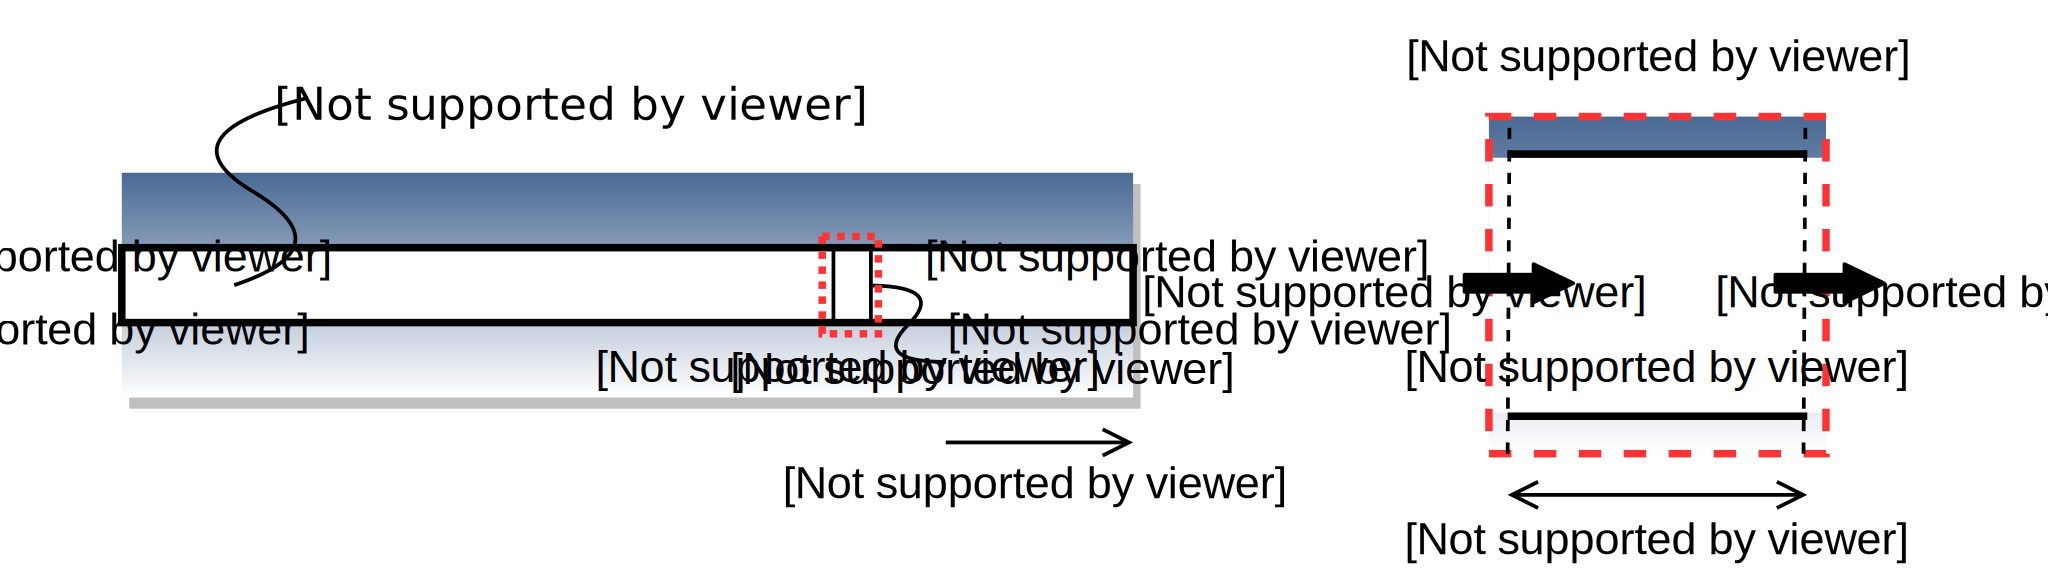
\includegraphics[width=16cm]{plots/cond-rod.png}
\caption{Conduction in a rod with internal heat production.}
\label{fig:conduction}
\end{figure}

We will take for the control volume a slice $dx$ from the rod.  The energy balance for the rod element $dx$:

\begin{equation}
\frac{dE_{dx}}{dt} = E_{dx, in} - E_{dx, out} + E_{dx, production}
\end{equation}

Note here that $E_{dx, in}$, $E_{dx, out}$ and $E_{dx, production}$ are energies per unit time and so have the units of $W$.

The heat flux $\phi$ which has units of $W$ can be modeled using the Fourier's law for one-dimensional heat conduction:

\begin{equation}
\phi = \lambda A \Big(- \frac{dT}{dx} \Big)
\label{eq:fourier}
\end{equation}

where $\lambda$ is the thermal conductivity and is a property of the material, $A$ is the rod's cross-sectional area and $\frac{dT}{dx}$ is a temperature gradient which plays a role of the driving force for thermal energy transport.

Hence:

\begin{equation}
E_{dx, in} = \lambda A \Big(- \frac{dT}{dx} \Big)_x
\end{equation}

\begin{equation}
E_{dx, out} = \lambda A \Big(- \frac{dT}{dx} \Big)_{x + dx}
\end{equation}

The energy per unit time coming from the heat production can be written as $Q_p$ multiplied by the volume of the slice $dx$:

\begin{equation}
E_{dx, production} = Q_p A dx
\end{equation}

In the steady-state $\frac{dE}{dt} = 0$ and the energy balance becomes:

\begin{equation}
\lambda A \Big(- \frac{dT}{dx} \Big)_x - \lambda A \Big(- \frac{dT}{dx} \Big)_{x + dx} + Q_p A dx = 0
\end{equation}

Simplifying the above energy balance we get:

\begin{equation*}
\frac{\Big(\frac{dT}{dx} \Big)_{x + dx} - \Big(\frac{dT}{dx} \Big)_x  }{dx} = - \frac{Q_p}{\lambda}
\end{equation*}

It is interesting to note here that we have lost the dependence on the cross-sectional surface area of the rod.

If we now substitute some function $f(x) = \frac{dT}{dx}$ we notice that we have:

\begin{equation*}
\frac{f(x + dx) - f(x)}{dx} = - \frac{Q_p}{\lambda}
\end{equation*}

in other words:

\begin{equation}
\frac{df(x)}{dx} = - \frac{Q_p}{\lambda}
\end{equation}

With the above substitution, the differential equation that we are about to solve becomes:

\begin{equation}
\frac{d^2T}{dx^2} = - \frac{Q_p}{\lambda}
\end{equation}

Applying the boundary conditions from both ends of the rod, the solution to the above differential equation is:

\begin{equation}
T(x) = - \frac{Q_p}{2 \lambda} (x^2 - Lx) + T_0
\label{eq:solution}
\end{equation}

\subsection{Final remarks}

Note that even though the heat flow was assumed to be one-dimensional in this exercise, it does not mean that the geometry of the problem needs to be one-dimensional. In fact, we assumed the rod to be a three-dimensional object having length and a cross-sectional area. Rather, the one-dimensionality of the problem means that it is practical to assume only one of the three directions as an important direction for heat transport. Since the rod was perfectly insulated along its length, the temperature gradient along directions perpendicular to the $x$-axis is zero.

\subsection{Computational example}

As a computational example we will draw the graph of the temperature distribution in a copper rod $200 m$ long. We assume that the thermal conductivity for this rod is $400 \frac{W}{m \cdot K}$. The internal heat production in the entire rod is $20 W$.

\begin{figure}[H]
\centering\includegraphics[width=16cm]{Code/conduction-rod.png}
\caption{Temperature distribution in a rod with internal heat production of $20 W$.}
\label{fig:python_graph}
\end{figure}

\newpage

\section{Steady-state laminar flows of Newtonian fluids}

The derivation of the velocity distribution in a steady-state laminar flow of a Newtonian fluid starts with writing the equation for momentum transport between the fluid \textit{laminates}.

\subsection{Couette flow}


\subsection{Poiseuille flow}

Consider a steady-state flow of fluid between two parallel plates. We would like to find the velocity and shear stress distribution along the $y$-axis.The pressure drop is assumed to be constant throughout the channel. This means that the pressure is a function of position $p = p(x)$ but the change in pressure per every equal distance in the channel is constant: $dp/dx = \text{const}$. The width of the channel $B$ is much larger compared to its other dimensions.

\begin{figure}[H]
\centering\includegraphics[width=15cm]{plots/poiseuille-fluid-element.png}
\caption{Flow between two parallel plates with an infinitesimal fluid element.}			
\label{fig:poiseuille-fluid-element}
\end{figure}

We also have three boundary conditions. Due to a no-slip condition we assume that the velocity at the very surface of the plates is zero: $u(-D/2) = 0$ and $u(D/2) = 0$. Due to symmetry of the flow we assume that there cannot be any net momentum transfer between the upper half and the lower half of the channel. Hence, the shear stress exactly in the middle of the channel is zero: $\tau_{xy}(0) = 0$.

Steady state momentum (force) balance, taking into account pressure and shear forces on a single infinitesimal fluid element:

\begin{equation}
0 = p|_x B dy - p|_{x+dx} B dy + \tau_{xy}|_y B dx - \tau_{yx}|_{y+dy} B dx
\end{equation}

Dividing both sides by the width $B$ and by $dx dy$ we obtain:

\begin{equation}
0 = \frac{p|_x  - p|_{x+dx}}{dx}  + \frac{\tau_{xy}|_y  - \tau_{yx}|_{y+dy}}{dy} 
\end{equation}

Now we notice that $\frac{p|_x  - p|_{x+dx}}{dx}$ is in fact equal to $-\frac{dp}{dx}$ (in a limit as $dx \rightarrow 0$), since it is an incremental change in pressure function value per incremental distance $dx$. Similar thing can be said about $\frac{\tau_{xy}|_y  - \tau_{yx}|_{y+dy}}{dy}$ which is equal to $-\frac{d \tau_{xy}}{dy}$. We can thus further simplify:

\begin{equation}
\frac{d \tau_{xy}}{dy} = - \frac{dp}{dx} = \text{const}
\end{equation}

Integrating the above equation and applying the initial condition for the shear stress $\tau_{xy}(0) = 0$:

\begin{equation} \label{eq:shear-poiseuille}
\tau_{xy}(y)= - \frac{dp}{dx} y
\end{equation}

Adding a constitutive relation for Newtonian fluids we can further relate pressure and velocity. From the Newton's law we know also that:

\begin{equation} \label{eq:shear-newton}
\tau_{xy}(y)= - \mu \frac{du}{dy}
\end{equation}

You may look at this in such a way: the equation \ref{eq:shear-poiseuille} is a special case in which the shear stresses have been related to the driving force in the Poiseuille flow - the pressure gradient. The equation \ref{eq:shear-newton} is a general description of any shear stress $\tau_{xy}$, where it is linked to velocity gradients, no matter what the cause for this velocity gradient is! It just so happens that in the case of a Poiseuille flow between two parallel plates this cause is the pressure drop:

\begin{equation}
- \mu \frac{du}{dy} = - \frac{dp}{dx} y
\end{equation}

Integrating one more time the above relation and applying the no-slip boundary conditions we get:

\begin{equation}
u(y) = \frac{1}{2 \mu} \frac{dp}{dx} (y^2 - (D/2)^2)
\end{equation}


\newpage

\section{Lumped system analysis of a steel plate}

In a lumped system analysis, we assume that the temperature of the body changes only with time and is independent of position inside the body. As you might already anticipate, this restriction cannot be applicable to every transient heat transfer problem, as in the majority of applications the temperature does change also with position. Regardless, this model might be useful in some cases and is therefore worth adding to your toolbox.

We start with stating that:

\begin{equation} \label{lumped-system-text}
\text{heat transfered to the body in during $dt$} = \text{change in internal energy of the body during $dt$}
\end{equation}

The heat transfer is modeled via the Fick's law:

\begin{equation}
\dot{Q} = h A_s (T_{\infty} - T(t))
\end{equation}

Note here that if $T_{\infty} > T(t)$, the heat transfer will happen from the surroundings to the body.

The change in internal energy is:

\begin{equation}
\Delta E = m c_p \frac{dT}{dt}
\end{equation}

We can therefore write the equation (\ref{lumped-system-text}) as:

\begin{equation}
h A_s (T_{\infty} - T(t)) = m c_p \frac{dT}{dt}
\end{equation}










\newpage

\section{Evaporating sphere}

\begin{figure}[H]
\centering\includegraphics[width=16cm]{Code/evaporating-sphere.png}
\caption{Evaporating sphere diameter history.}
\label{fig:stefan-problem}
\end{figure}

\newpage

\section{One-dimensional binary diffusion}



\newpage

\section{The Stefan problem}

\begin{figure}[H]
\centering\includegraphics[width=16cm]{Code/stefan-problem.png}
\caption{Stefan problem for water evaporating from the 0.1m tube.}
\label{fig:stefan-problem}
\end{figure}




\newpage

\section{Batch reactor}

The general form of the continuity equation for species $i$ in the Eulerian form:

\begin{equation} \label{eq:species-mass-conservation}
\frac{\partial \rho \omega_i}{\partial t} = s_i - \nabla \rho \omega_i \mathbf{u}_{i}
\end{equation}

Where $\rho$ is the density of the mixture, $\omega_i$ is species mass fraction, $s_i$ is the production rate of species $i$ and $\mathbf{u}_i$ is the velocity of species $i$ in the mixture.

For a 0-D batch reactor we assume that the spatial gradients of any quantity are zero, and so: $ \nabla \rho \omega_i \mathbf{u}_{i} = 0$. The only possible changes inside the reactor will happen in time. Since the species mass fraction is only a function of time we can degrade the $\frac{\partial}{\partial t}$ derivative to $\frac{d}{dt}$. Also as a side note: $\rho \omega_i = m_i$ which is mass of species $i$ in the mixture. We can thus write:

\begin{equation} \label{eq:batch-reactor-species-mass}
\frac{d \omega_i}{dt} = \frac{s_i}{\rho}
\end{equation}

assuming that the density is constant in time.

We are going to use the $1^{st}$ law of thermodynamics:

\begin{equation}
\frac{dU}{dt} = \frac{dQ}{dt} + \frac{dW}{dt}
\end{equation}

and we will substitute something for $\frac{dU}{dt}$ and $\frac{dW}{dt}$.

We know that the total enthalpy:

\begin{equation}
H = U + p V
\end{equation}

and differentiating that with respect to time gives:

\begin{equation} \label{eq:enthalpy}
\frac{d H}{dt} = \frac{dU}{dt} + p \frac{dV}{dt} + V \frac{dp}{dt}
\end{equation}

We also know that:

\begin{equation} \label{eq:power}
\frac{dW}{dt} = -p \frac{dV}{dt}
\end{equation}


Substituting eq.(\ref{eq:power}) and eq.(\ref{eq:enthalpy}) into the $1^{st}$ law of thermodynamics we get:

\begin{equation}
\frac{dH}{dt} - p \frac{dV}{dt} - V \frac{dp}{dt} = \frac{dQ}{dt} -p \frac{dV}{dt}
\end{equation}

Which then simplifies to:

\begin{equation} \label{eq:enthalpy-from-1st-law}
\frac{dH}{dt}  = \frac{dQ}{dt} + V \frac{dp}{dt}
\end{equation}

We are now going to use the above equation in which we will substitute the expression for the time derivative of enthalpy $\frac{dH}{dt}$.

Writing the enthalpy as an extensive property in terms of the specific enthalpy:

\begin{equation}
H = m h = m \sum_{i=1}^n \omega_i h_i
\end{equation}

where $h_i = h_{f,i}^{(0)} + c_{p,i} \Delta T$ and $h_{f,i}^{(0)}$ is the enthalpy of formation at reference conditions and the term $c_{p,i} \Delta T$ accounts for temperature difference with respect to the reference temperature. In other words:

\begin{equation}
H = m \sum_{i=1}^n \omega_i ( h_{f,i}^{(0)} + c_{p,i} \Delta T )
\end{equation}

which we can differentiate with respect to time:

\begin{equation*}
\frac{dH}{dt} = m \frac{d}{dt} \sum_{i=1}^n \omega_i ( h_{f,i}^{(0)} + c_{p,i} \Delta T )
\end{equation*}

\begin{equation*}
\frac{dH}{dt} = m \sum_{i=1}^n  \frac{d \omega_i}{dt}  h_{f,i}^{(0)}  + m \sum_{i=1}^n \frac{d}{dt} ( \omega_i c_{p,i} \Delta T )
\end{equation*}

\begin{equation*}
\frac{dH}{dt} = m \sum_{i=1}^n  \frac{d \omega_i}{dt}  h_{f,i}^{(0)}  + m \sum_{i=1}^n \frac{d}{dt} ( \omega_i c_{p,i} (T(t) - T_{ref}) )
\end{equation*}

\begin{equation*}
\frac{dH}{dt} = m \sum_{i=1}^n  \frac{d \omega_i}{dt}  h_{f,i}^{(0)}  + m \sum_{i=1}^n \frac{d \omega_i}{dt} c_{p,i} T(t) + m \sum_{i=1}^n \omega_i c_{p,i} \frac{d T(t)}{dt}  - m \sum_{i=1}^n \frac{d \omega_i}{dt} c_{p,i} T_{ref}
\end{equation*}

We can now substitute eq.(\ref{eq:species-mass-conservation}) into all terms  representing $\frac{d \omega_i}{dt}$:

\begin{equation*}
\frac{dH}{dt} = m \sum_{i=1}^n  \frac{s_i}{\rho}  h_{f,i}^{(0)}  + m \sum_{i=1}^n \frac{s_i}{\rho} c_{p,i} T(t) + m \sum_{i=1}^n \omega_i c_{p,i} \frac{d T(t)}{dt}  - m \sum_{i=1}^n \frac{s_i}{\rho} c_{p,i} T_{ref}
\end{equation*}

Recognize also that $\frac{d T(t)}{dt}$ is independent of the species and can be factored out in the summation, and that $\sum_{i=1}^n \omega_i c_{p,i} = c_p$ for the entire mixture by definition. Rearranging the terms we get:

\begin{equation*}
\frac{dH}{dt} = m c_{p} \frac{d T(t)}{dt} + m \sum_{i=1}^n  \frac{s_i}{\rho}  ( h_{f,i}^{(0)} + c_{p,i} T(t)  - c_{p,i} T_{ref})
\end{equation*}

At this point we can also recognize that the density can be factored out of summation and combined with the total mass of the mixture to give the total volume. We get finally:

\begin{equation} \label{eq:differentiated-enthalpy}
\frac{dH}{dt} = m c_{p} \frac{d T(t)}{dt} + V \sum_{i=1}^n  s_i  h_i
\end{equation}

We can now combine eq.(\ref{eq:enthalpy-from-1st-law}) and eq.(\ref{eq:differentiated-enthalpy}) to obtain:

\begin{equation} 
\frac{dQ}{dt} + V \frac{dp}{dt} = m c_{p} \frac{d T(t)}{dt} + V \sum_{i=1}^n  s_i h_i
\end{equation}

Rearranging terms we get the general expression for temperature change in the batch reactor:

\begin{equation} \label{eq:bath-reactor-energy}
m c_{p} \frac{d T(t)}{dt}  = \frac{dQ}{dt} + V \frac{dp}{dt} - V \sum_{i=1}^n  s_i  h_i 
\end{equation}

The above equation assumes that temperature $T$, volume $V$, pressure $p$ and heat $Q$ can be functions of time. Restricting any of those terms we may however arrive at special cases of the batch reactor equations. We present next one of such special cases.


\newpage

\subsection{Closed, adiabatic, constant pressure batch reactor}

For a closed, adiabatic $\frac{dQ}{dt} = 0$ and constant pressure $\frac{dp}{dt}= 0$ batch reactor we can simplify eq.(\ref{eq:bath-reactor-energy}):

\begin{equation} \label{eq:bath-reactor-adiabatic-constant-pressure}
 \frac{d T(t)}{dt}  = - \frac{1}{\rho c_{p}} \sum_{i=1}^n  s_i  h_i 
\end{equation}

Notice that this equation resembles eq.(\ref{eq:batch-reactor-species-mass}) and sometimes you may find both of these equations written in the form:

\begin{equation} \label{eq:bath-reactor-adiabatic-constant-pressure}
 \frac{d \boldsymbol{\phi}}{dt}  = \mathbf{s}_{\phi}
\end{equation}

\begin{equation} \label{eq:bath-reactor-adiabatic-constant-pressure}
\mathbf{s}_{\eta} = \mathbf{s}_{\phi} \mathbf{A} \mathbf{D}^{-1}
\end{equation}


where $ \boldsymbol{\phi} = [T, \omega_1, \omega_2, \dots \omega_n]$ and $s_{\phi}$ is a \textit{production rate} of $\phi$. The production rate is equal to $\frac{s_i}{\rho}$ if $\phi_i = \omega_i$ and it is equal to $ - \frac{1}{\rho c_{p}} \sum_{i=1}^n  s_i  h_i $ when $\phi_i = T$. It is worth pointing out that for the temperature, the production rate is actually a sum of production rates of all the species multiplied by their enthalpies. This is in contrast to eq.(\ref{eq:batch-reactor-species-mass}), where for each $\omega_i$ only one corresponding $s_i$ appears in a differential equation.







\subsection*{References}

A. Parente, \textit{Heat Transfer and Combustion}, Université libre de Bruxelles, 2019

J. C. Sutherland, \textit{Multicomponent Mass Transfer}, CHEN 6603, The University of Utah, 2012




\end{document}